\begin{frame}{Cellule d'un LSTM}
    
    \begin{columns}
        \begin{column}{.47\textwidth}
            \begin{itemize}
                \item Cellule mémoire au centre
                \item Portes controllant le flux d'information entrant / sortant / restant dans la cellule.
                \item Permettent de conserver de l'information durablement si besoin.
                \item Peuvent être vues comme des opérations :
                   \begin{itemize}
                        \item Ecriture \textit{(input gate)}
                        \item Lecture \textit{(output gate)}
                        \item Réinitialisation \textit{(forget gate)}
                    \end{itemize}
            \end{itemize}
            
            
        \end{column}
        \begin{column}{.55\textwidth}
            \begin{figure}
                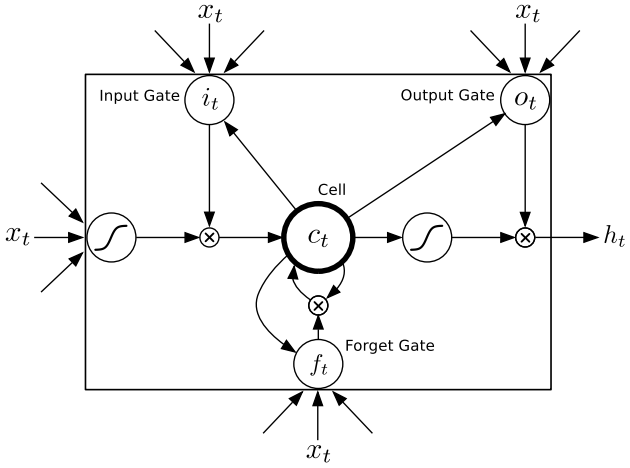
\includegraphics[width=\textwidth]{images/lstm4}
                \caption{Cellule LSTM {\scriptsize\it -- Source : \cite{Graves13b}}}
            \end{figure}
        \end{column}
    \end{columns}
    
\end{frame}

\begin{frame}{Exemple de comportement possible}
    
    \begin{figure}
        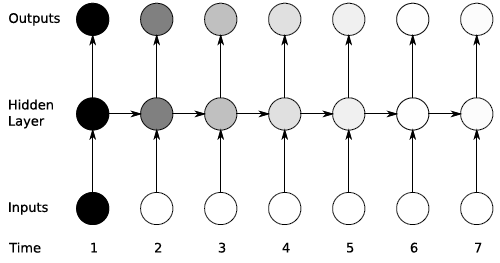
\includegraphics[height=.35\textheight]{images/res_rnn}
        \vspace{-.4cm}
        \caption{Exemple pour un RNN {\scriptsize\it -- Source : \cite{Graves12}}}
    \end{figure}
    
    \vspace{-.5cm}
    
    \begin{figure}
        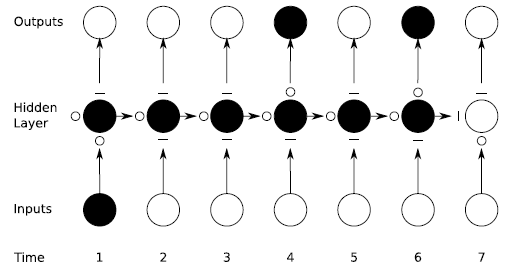
\includegraphics[height=.35\textheight]{images/res_lstm}
        \vspace{-.4cm}
        \caption{Exemple pour un LSTM {\scriptsize\it -- Source : \cite{Graves12}}}
    \end{figure}
    
\end{frame}



